% ==============================================================================
\section{Background \& High-Level Write Strategies}
\label{sec:background}
% ==============================================================================

\subsection{Parallel File Systems and Data Striping}
\label{sec:pfs}

Traditional file systems rely on single storage controllers, which creates a severe bottleneck 
when thousands of parallel MPI ranks attempt simultaneous file access. PFS—such as Lustre, BeeGFS, 
and many others—bypass this bottleneck by partitioning files across multiple independent storage devices via data striping.

In such systems, storage capacity is divided into logical entities called Object Storage Targets 
(OSTs). An OST represents a dedicated physical storage unit (e.g., a RAID array or NVMe volume) managed 
by an Object Storage Server (OSS). Metadata servers (MDS) maintain directory structures and file layouts, 
while OSTs handle actual data payload transfers.

Data striping partitions a logical file stream into contiguous blocks of size $S_{\text{stripe}}$ (Stripe Size). 
These blocks are distributed in a round-robin sequence across $N_{\text{OST}}$ targets (Stripe Count or OST Count). 
For example, with $N_{\text{OST}} = 4$ and $S_{\text{stripe}} = 1$~MB, the first megabyte is written to OST~0, the second 
to OST~1, and so on. Striping allows applications to aggregate the physical bandwidth of multiple storage devices, ideally 
achieving an $N_{\text{OST}}$-fold increase in overall write throughput.

\subsection{Parallel Write Strategies}
\label{sec:strategies}

The layout of output files significantly impacts storage efficiency. In this study, we analyze three primary high-level I/O strategies, 
implemented via the Parallel Data Interface (PDI) middleware:

\subsubsection{Single Shared File}
In the Single Shared File approach, all MPI processes concurrently write their local data slices into a single unified file on the PFS 
(Figure~\ref{fig:ssf_schema}). Standard libraries (such as HDF5 or MPI-IO) employ two-phase I/O to aggregate non-contiguous memory layouts 
into large, contiguous file offsets before issuing collective storage calls. While SSF simplifies dataset management by producing a single 
output file, it can suffer from locking contention on storage targets when rank counts scale up.

\begin{figure}[h]
  \centering
  \definecolor{rouge_inria}{RGB}{180,0,0}

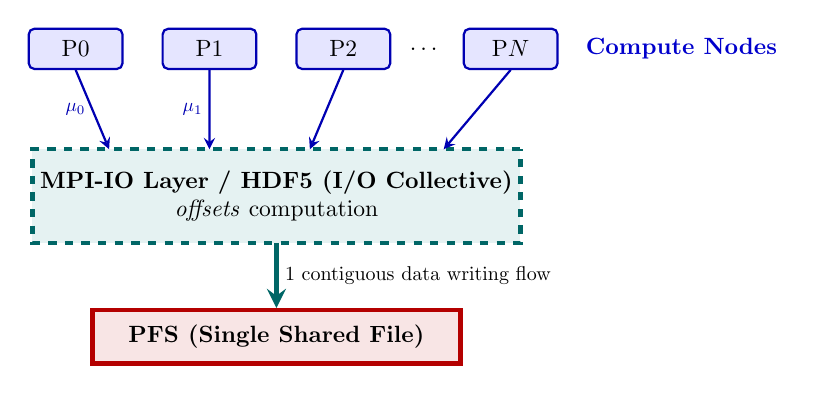
\begin{tikzpicture}[
    scale=0.85, every node/.style={transform shape},
% Block styles
    mpi/.style={rectangle, draw=blue!70!black, fill=blue!10, thick, minimum width=1.4cm, minimum height=0.6cm, rounded corners=2pt},
    agg/.style={rectangle, draw=teal!80!black, fill=teal!10, dashed, ultra thick, minimum width=6.5cm, minimum height=1.4cm, align=center},
    pfs/.style={rectangle, draw=rouge_inria, fill=rouge_inria!10, ultra thick, minimum width=5.5cm, minimum height=0.8cm, align=center}
]

% 1. Processes (data scattered in memory)
\node[mpi] (mpi0) at (-3, 2.5) {P0};
\node[mpi] (mpi1) at (-1, 2.5) {P1};
\node[mpi] (mpi2) at (1, 2.5) {P2};
\node (mpidots) at (2.2, 2.5) {$\dots$};
\node[mpi] (mpiN) at (3.5, 2.5) {P$N$};
\node[anchor=west, text=blue!80!black] at (4.5, 2.5) {\textbf{Compute Nodes}};

% 2. Aggregation step (collective I/O)
\node[agg] (aggregation) at (0, 0.3) {\textbf{MPI-IO Layer / HDF5 (I/O Collective)}\\ \textit{offsets} computation};

% Arrows processes -> aggregation
\draw[->, >=stealth, thick, blue!70!black] (mpi0.south) -- (-2.5, 1) node[midway, left, scale=0.8] {$\mu_0$};
\draw[->, >=stealth, thick, blue!70!black] (mpi1.south) -- (-1, 1) node[midway, left, scale=0.8] {$\mu_1$};
\draw[->, >=stealth, thick, blue!70!black] (mpi2.south) -- (0.5, 1);
\draw[->, >=stealth, thick, blue!70!black] (mpiN.south) -- (2.5, 1);

% 3. Single write to the PFS
\node[pfs] (pfsfile) at (0, -1.8) {\textbf{PFS (Single Shared File)}};

% Single contiguous write flow
\draw[->, >=stealth, line width=2pt, teal!80!black] (0, -0.4) -- (pfsfile.north) 
        node[midway, right, text=black, scale=0.85] {1 contiguous data writing flow};

\end{tikzpicture}
  \caption{Single Shared File strategy overview.}
  \label{fig:ssf_schema}
\end{figure}

\subsubsection{Subfiling}
Subfiling acts as an intermediate approach between SSF and individual file writes. MPI processes are partitioned into distinct sub-groups. 
Within each group, an assigned process—referred to as an I/O Concentrator (IOC) or aggregator—collects data from its peer ranks and writes 
it to a dedicated subfile (Figure~\ref{fig:subfiling_schema}). 

This reduces file system lock contention compared to SSF, while avoiding the metadata overload associated with generating thousands of individual 
files. The total number of generated subfiles ($N_{\text{subfiles}}$) is a tunable parameter.

\begin{figure}[h]
  \centering
  \definecolor{rouge_inria}{RGB}{180,0,0}

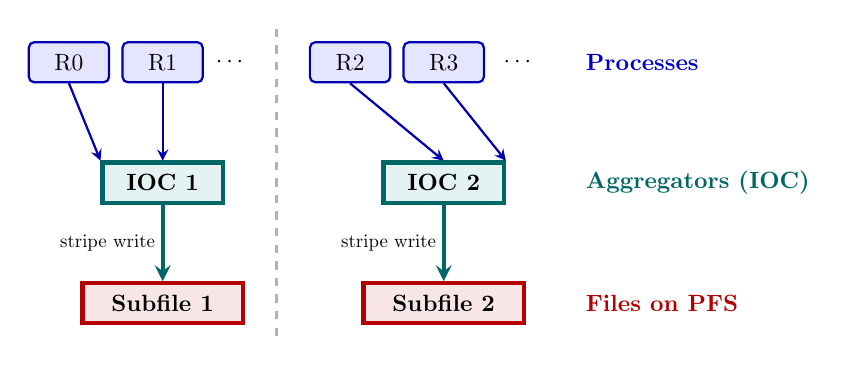
\begin{tikzpicture}[
    scale=0.85, every node/.style={transform shape},
    mpi/.style={rectangle, draw=blue!70!black, fill=blue!10, thick,
                minimum width=1.2cm, minimum height=0.6cm, rounded corners=2pt},
    ioc/.style={rectangle, draw=teal!80!black, fill=teal!10, ultra thick,
                minimum width=1.8cm, minimum height=0.6cm, align=center},
    sub/.style={rectangle, draw=rouge_inria, fill=rouge_inria!10, ultra thick,
                minimum width=2.4cm, minimum height=0.6cm, align=center}
]
 
    % Group 1 ranks
    \node[mpi] (m0) at (-3.8, 3) {R0};
    \node[mpi] (m1) at (-2.4, 3) {R1};
    \node      at   (-1.4, 3)    {$\cdots$};
 
    % Group 2 ranks
    \node[mpi] (m2) at ( 0.4, 3) {R2};
    \node[mpi] (m3) at ( 1.8, 3) {R3};
    \node      at   ( 2.9, 3)    {$\cdots$};
 
    \node[anchor=west, text=blue!80!black, font=\bfseries] at (3.8, 3) {Processes};
 
    % Group separating dashed line
    \draw[dashed, gray!60, thick] (-0.7, 3.5) -- (-0.7, -1.2);
 
    % IOC nodes
    \node[ioc] (ioc1) at (-2.4, 1.2) {\textbf{IOC 1}};
    \node[ioc] (ioc2) at ( 1.8, 1.2) {\textbf{IOC 2}};
    \node[anchor=west, text=teal!80!black, font=\bfseries] at (3.8, 1.2)
        {Aggregators (IOC)};
 
    % Arrows Ranks -> IOC
    \draw[->, >=stealth, thick, blue!70!black] (m0.south) -- (ioc1.north west);
    \draw[->, >=stealth, thick, blue!70!black] (m1.south) -- (ioc1.north);
    \draw[->, >=stealth, thick, blue!70!black] (m2.south) -- (ioc2.north);
    \draw[->, >=stealth, thick, blue!70!black] (m3.south) -- (ioc2.north east);
 
    % Subfiles
    \node[sub] (f1) at (-2.4, -0.6) {\textbf{Subfile 1}};
    \node[sub] (f2) at ( 1.8, -0.6) {\textbf{Subfile 2}};
    \node[anchor=west, text=rouge_inria, font=\bfseries] at (3.8, -0.6)
        {Files on PFS};
 
    % Arrows IOC -> Subfiles
    \draw[->, >=stealth, line width=1.5pt, teal!80!black]
        (ioc1.south) -- (f1.north)
        node[midway, left, scale=0.8, text=black] {stripe write};
    \draw[->, >=stealth, line width=1.5pt, teal!80!black]
        (ioc2.south) -- (f2.north)
        node[midway, left, scale=0.8, text=black] {stripe write};
 
\end{tikzpicture}
  \caption{Subfiling strategy overview with two I/O Concentrators (IOCs).}
  \label{fig:subfiling_schema}
\end{figure}

\subsubsection{File Per Process }
\label{fig:fpp_schema}
In the File Per Process approach, every MPI process creates and writes its own separate file independently (Figure~\ref{fig:fpp_schema}). Because there is 
no inter-process communication or offset synchronization required, local write throughput can be very high. However, FPP generates $N_{\text{ranks}}$ separate 
files per checkpoint, which can strain metadata servers (MDS) at scale and complicate downstream post-processing or data management.

\begin{figure}[h]
  \centering
  \definecolor{rouge_inria}{RGB}{180,0,0}

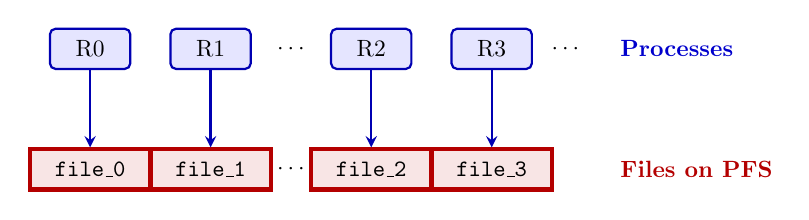
\begin{tikzpicture}[
    scale=0.85, every node/.style={transform shape},
    mpi/.style={rectangle, draw=blue!70!black, fill=blue!10, thick,
                minimum width=1.2cm, minimum height=0.6cm, rounded corners=2pt},
    pfs/.style={rectangle, draw=rouge_inria, fill=rouge_inria!10, ultra thick,
                minimum width=1.8cm, minimum height=0.6cm, align=center}
]
 
    % MPI Ranks
    \node[mpi] (m0) at (-3.8, 3) {R0};
    \node[mpi] (m1) at (-2.0, 3) {R1};
    \node      at   (-0.8,  3)   {$\cdots$};
    \node[mpi] (m2) at ( 0.4, 3) {R2};
    \node[mpi] (m3) at ( 2.2, 3) {R3};
    \node      at   ( 3.3,  3)   {$\cdots$};
    \node[anchor=west, text=blue!80!black, font=\bfseries] at (4.0, 3) {Processes};
 
    % Per-process files
    \node[pfs] (f0) at (-3.8, 1.2) {\texttt{file\_0}};
    \node[pfs] (f1) at (-2.0, 1.2) {\texttt{file\_1}};
    \node      at   (-0.8,  1.2)   {$\cdots$};
    \node[pfs] (f2) at ( 0.4, 1.2) {\texttt{file\_2}};
    \node[pfs] (f3) at ( 2.2, 1.2) {\texttt{file\_3}};
    \node[anchor=west, text=rouge_inria, font=\bfseries] at (4.0, 1.2)
        {Files on PFS};
 
    % Direct arrows Rank -> File (no coordination)
    \draw[->, >=stealth, thick, blue!70!black] (m0.south) -- (f0.north);
    \draw[->, >=stealth, thick, blue!70!black] (m1.south) -- (f1.north);
    \draw[->, >=stealth, thick, blue!70!black] (m2.south) -- (f2.north);
    \draw[->, >=stealth, thick, blue!70!black] (m3.south) -- (f3.north);
     
\end{tikzpicture}
  \caption{File Per Process  strategy overview.}
\end{figure}

\subsection{Software Stack and Tooling}
\label{sec:tools}

To evaluate these strategies, our experimental framework combines three key software components:

\begin{itemize}
    \item \textbf{gys\_io Mini-App:} Developed by CEA, gys\_io is a lightweight benchmark proxy that replicates Gysela's exact 5D domain decomposition and checkpoint write calls while skipping computational physics routines. It reads Gysela configuration files directly, enabling fast, reproducible I/O benchmarks.
    \item \textbf{Parallel Data Interface (PDI):} PDI decouples application code from underlying I/O libraries. By modifying external YAML configuration files, PDI allows switching between SSF, Subfiling, and FPP backends without recompiling the application binary.
    \item \textbf{IOPS Benchmark Automation:} IOPS automates parameter sweeps, manages SLURM batch job submission, and extracts execution metrics (such as \texttt{time\_write} and aggregate write bandwidth). 
\end{itemize}


